% ---------------------------------
% Introduction
% ---------------------------------
\section{Introduction}
For my project, I implemented a parallel brute force N-Body Simulation which runs in $O(n^2)$ time.
The brute force approach is often times called the ``all-pairs N-body simulation'' as it simulates
the interaction between all the pairs of bodies in the simulation, while other methods,
such as the Barnes-Hut simulation, achieve better performance by approximating the interaction
by reducing the number of interactions based on the distance between two bodies.\\
\indent N-Body Simulations can be used to model the interaction between many different things, such as
planets, galaxies, and particles. My simulation models the interaction between bodies exerting
a gravitational force on one another, with a very large and dense mass being in the middle that also
exerts a force on every body in the simulation. \\
\indent The acceleration of a body due to the gravitational force exerted on it by another body 
can be modeled by the following equation: 
\begin{equation}
    a_i \approx G \cdot \sum\limits_{j=1}{^N}\frac{m_j \cdot \vec{r_{ij}}}{(\left\lVert\vec{r_{ij}}\right\rVert^2 + \epsilon^2)^\frac{3}{2}} \label{sec:grav}
\end{equation}
The $\epsilon$ is known as a softening factor and is set to $1 \times 10^{-8}$ in order to prevent 
division by zero and not have particles collide, but rather pass through each other.
My simulation uses this equation to update the velocity of each particle over a small time-step $dt = 0.01$
by multiplying the result $a_i$ by the time-step $dt$. \\
\indent I have tested multiple different implementations of the brute-force algorithm. 
They include sequential CPU code, OpenMP parallelized CPU code, basic CUDA code 
(this is just a direct port of the sequential CPU code to a CUDA kernel),
and optimized CUDA code using shared memory and loop unrolling.
Both of the CUDA versions use structures of arrays, \verb|float4|s, and a compiler flag that flushes 
denormal numbers to zero (more on this later) to achieve the most optimal speed. \\
\indent Times were recorded in milliseconds using the \verb|high_resolution_clock| from 
the \verb|<chrono>| library from the \verb|C++| STL. For the CPU 
implementation, the timer was started before the function that handled the simulation was called and
was ended as soon as the function returned. For the CUDA implementation, the timer was started before
the kernel was called and was ended as soon as the kernel returned (before memory was copied from the 
device to the host). The time reported is the amount of time each function/kernel call took
averaged over 10 total calls, and the first CUDA kernel launch is ignored since it always 
takes significantly longer due to the overhead of setting up the device for the first call.\\
\indent Each body's initial position and velocity was initialized randomly using the \verb|<random>| library's 
\verb|uniform_int_distribution<T>| class functionality.\\
\indent The simulation, timing scripts, checkers, and \LaTeX  code for this report
in available on \href{https://github.com/robertfeliciano/nbody}{GitHub}.

\section{Hardware Specifications} 
The simulation was run locally on my Windows 10 PC using WSL2. The specifications are the following:
\begin{itemize}
    \item CPU: AMD Ryzen 5 5600X, 6-core, 12-Thread
    \item GPU: NVIDIA GeForce RTX 3070 Ti
\end{itemize}
These specifications are important as different CPUs will experience different speed-ups
from OpenMP depending on how many threads are available. Along with that, different GPUs
will also experience different speeds based on factors such as their streaming multiprocessor
count.

\section{Suitability for GPU Acceleration - Amdahl's Law}
Since the interaction between one pair of bodies is completely independent from the 
interaction between another pair of bodies, this problem is embarrassingly parallel. 
The entire computation can be parallelized on the GPU. Unlike the versions showed in 
class that updated each body's position vector on the CPU, the implementations 
discussed in this report have the entire computation on the GPU or in the OpenMP 
parallelized for-loop. With these implementations, we achieve 100\% parallelism for simulating
the interaction between all N bodies.

\section{CPU Implementations}
The sequential implementation of the brute-force simulation is very simple. There are two
for-loops with one nested in the other:
\begin{lstlisting}[
    language=C++,
    basicstyle=\ttfamily\small,
    keywordstyle=\color{blue}\ttfamily,
    stringstyle=\color{red}\ttfamily,
    aboveskip=1em,
    belowskip=1em,
    lineskip=0.5em]
    for (int i = 0; i < n; i++){
        float fx = 0.0f, fy = 0.0f, fz = 0.0f;
        for (int j = 0; j < n; j++){
            float dx = b[j].x - b[i].x;
            // code continues...
\end{lstlisting}
This sequential version of the code is very slow. Thanks to OpenMP, 
we can easily parallelize this by putting a \verb|#pragma omp parallel for schedule(dynamic)| directive above the outer loop. 
This will spawn some number of threads, depending on how many are available on the CPU, and 
significantly speed up the simulation. By doing this, each thread calculates approximately \verb|N|/\verb|num_threads|
interactions rather than a single thread calculating every interaction (as it did in the original code). \\
\indent The rest of the code is trivial and simply implements \hyperref[sec:grav]{equation 1.1}. It computes the 
Euclidean distance between the each pair of bodies and uses that to find the force of attraction between each pair. 
Each body's force vector is updated for every other body. 
\begin{lstlisting}[
    language=C++,
    basicstyle=\ttfamily\small,
    keywordstyle=\color{blue}\ttfamily,
    stringstyle=\color{red}\ttfamily,
    aboveskip=1em,
    belowskip=1em,
    lineskip=0.5em]
    float dx = b[j].x - b[i].x;
    float dy = b[j].y - b[i].y;
    float dz = b[j].z - b[i].z;
    float d = dx*dx + dy*dy + dz*dz + EPSILON * EPSILON;
    float denom = 1.0f / sqrtf(d);
    float denom_cubed = denom * denom * denom;

    float m_j = b[j].m

    fx += m_j * dx * denom_cubed; 
    fy += m_j * dy * denom_cubed; 
    fz += m_j * dz * denom_cubed;
\end{lstlisting}
Finally, the force of attraction between a body and the large, dense mass in the middle is computed. 
The code then integrates the force over the small time-step $dt$ 
and multiplies by the gravitational constant ($G = 6.67 \times 10^{-11}$) to find the acceleration due to the force and adds this 
to the velocity vector. The velocity vector is then multiplied by $dt$ and used to update the position vector.
\begin{lstlisting}[
    language=C++,
    basicstyle=\ttfamily\small,
    keywordstyle=\color{blue}\ttfamily,
    stringstyle=\color{red}\ttfamily,
    aboveskip=1em,
    belowskip=1em,
    lineskip=0.5em]
    // dx, dy, dz, and denom_cubed re-calculated for center mass...
    m_c = center_obj.m
    fx -= m_c * dx * denom_cubed; 
    fy -= m_c * dy * denom_cubed; 
    fz -= m_c * dz * denom_cubed;

    b[i].vx += dt*fx*G;
    b[i].vy += dt*fy*G;
    b[i].vz += dt*fz*G;

    b[i].x += dt * b[i].vx;
    b[i].y += dt * b[i].vy;
    b[i].z += dt * b[i].vz;
\end{lstlisting}
\indent The code presented in class on May 3rd was very similar to this except I was updating the positions outside of the 
parallelized loop by using OpenMP's SIMD pragma directive (I simply added \verb|#pragma omp simd| above a 
loop that iterated over every body and updated each body's position vector). This was because I was experiencing a bug 
when I would update the positions in parallel on the GPU, so decided to use SIMD for both implementations. After fixing that bug 
and moving the position update inside the parallelized loop
I've noticed a slight increase in performance, but not too significant. \\
\indent Something interesting I discovered prior to updating the positions in parallel 
was that compiling the \verb|C++| code with the \verb|-O3| flag to 
optimize the code as much as possible led to no difference when adding \verb|#pragma omp simd|. 
Afer some research, I found out the loop I had originally was being automatically vectorized by the compiler due to the \verb|-O3| 
flag turning on the \verb|-ftree-vectorize| flag. I believe understanding more about how compilers optimize our 
code, oftentimes even better than any human could, is crucial to being a good programmer.\\

\section{CUDA Occupancy}
Before discussing the GPU implementations, I feel it is important to discuss the CUDA Occupancy achieved in them. 
I use a total of 12,288 bytes of shared memory since each block utilizes a shared array of 
768 (this is the block size) \verb|float4|s, each having a size of 16 bytes. Using the CUDA Occupancy calculator (CITE LEI MAO HERE)
I was able to determine that my implementation is at 100\% occupancy. \\
PUT THE STUFF WITH THE GRAPHS FROM THE SHEET HERE AND STUFF HERE \\
\indent I originally was using 1024 threads per block, which increased the shared memory size per block to be 16,384 bytes. However, 
using the occupancy calculator I discovered this was only utilizing 67\% occupancy. After switching from 1024 threads per block
to 768, I noticed a consistent 1 to 2 millisecond speed up when simulating 30,000 bodies. This speed up scaled appropriately while increasing 
the number of bodies, sometimes saving about a full second or two when N grew to 1 million bodies.

\section{GPU Implementations}
There were two GPU implementations written for this project: one was a simple port of the inner loop from the CPU code to a CUDA kernel and the other was a more optimized
algorithm that uses shared memory and loop unrolling. Since the simple version is very similar to the CPU code explained above, we will not discuss it here. \\
\indent The kernel begins by determining the global thread ID. Then, the code iterates over every block in the grid using a for-loop and, for each block, populates an array in shared memory for every thread in the current block to load in their corresponding body's information:
\begin{lstlisting}[style = cudastyle]
    for (int t = 0; t < gridDim.x; t++)
        __shared__ float4 others[BLOCKSZ];
        float4 curr = p[t * blockDim.x + threadIdx.x];
        // load other threads' info into shared memory
        // the "w field" is used to store the mass
        others[threadIdx.x] = make_float4(curr.x, curr.y, curr.z, curr.w);
        __syncthreads();
\end{lstlisting}
The code then iterates over the array and calculates the interaction between the body corresponding to the thread running the code (determined by the global thread ID) and every body in the array. This is very similar to the inner loop to the CPU version except for a \verb|#pragma unroll| placed above it so it will not be displayed here. One of the first thoughts I had was to launch another kernel from this one to parallelize this for-loop, but since each thread would be updating the same force I'd have to use atomic operations which would just slow it down anyway. Finally, something similar to the CPU code is done to calculate the ineraction between the current body and the large, dense center mass. The velocity vector is updated by calculating the acceleration from the force vector over $dt$ and similarly the position vector is updated by calculating the displacement from the velocity vector over $dt$.\\
\indent While I have not tested putting the bodies in constant memory, I believe my implementation may provide similar speeds or even greater since it requires only one kernel launch and uses shared memory. Also, using constant memory wouldn't work once the number of bodies surpasses $N = 2,048$. This is because each body has two \verb|float4|s to store its position, velocity, and mass which totals 32 bytes. Since constant memory is limited to 65,536 kilobytes, our number of bodies is also limited. This method, using a constant amount of shared memory per block ($768\;\text{bodies}\;\times\;16\;\text{bytes/body}\;=\;12,288\;\text{bytes}$) allows us to simulate any number of bodies.

\section{Other GPU Optimizations}
\indent There are three more optimizations I used to make the CUDA code as efficient as possible in both versions and they include the \verb|-ftz=True| compiler flag, using \verb|float4|s rather than regular floats, and using a structure of arrays. \\
\indent The CPU code uses an array of structures to represent the simulation, where each structure represents a body and has float fields for the body's x, y, z position and velocity and a field for its mass. The GPU code uses a single structure of arrays that represents the entire simulation. This structure has two \verb|float4| arrays, where the first array of \verb|float4|s stores each body's x, y, z position and mass, and the other stores each body's velocity. Using the structure of arrays enables greater memory coalescing and uses bandwidth more efficiently.\\
\indent \verb|Float4|s achieve better performance on the GPU because they utilize vectorized memory accesses \cite{Luitjens_2013}. Experiments have shown that using \verb|float4|s rather than regular floats can increase speeds by up to 25\% \cite{Vitality_2014}. The reason for this is twofold: "multi-word vector memory accesses only require a single instruction to be issued, so the bytes per instruction ratio is higher", and "vector sized transaction request from a warp results in a larger net memory throughput per transaction" \cite{talonmies_2015}. Therefore, by using \verb|float4|s I achieve significant speed-ups on top of using a structure of arrays.\\
\indent The \verb|-ftz=true| flag flushes what are known as "denormal values" to zero. This is by far the most interesting optimization I learned about while doing research for this project. Denormal values are floating point numbers where the mantissa is normalized and the leading zeros from it are moved into the exponent, resulting in an exponent that is too small and cannot be represented \cite{Harris_2013}. These numbers can slow down computation time significantly, especially for functions like \verb|sqrtf()| and \verb|rsqrtf()|. Since these numbers are so small, flushing them to zero does not affect accuracy at all. Using the \verb|-ftz=true| flag will flush all denormalized numbers to be flushed to zero, which doesn't have a performance impact on adds or multiplies but it does for functions like \verb|rsqrtf()| which map to hardware instructions, sometimes providing a 20\% speed increase \cite{Harris_2013}. I did not see this significant of a speed increase, but saw a small one nonetheless as shown in the figure below. 
\begin{figure}[H]
    \centering
    \makebox[\textwidth][c]{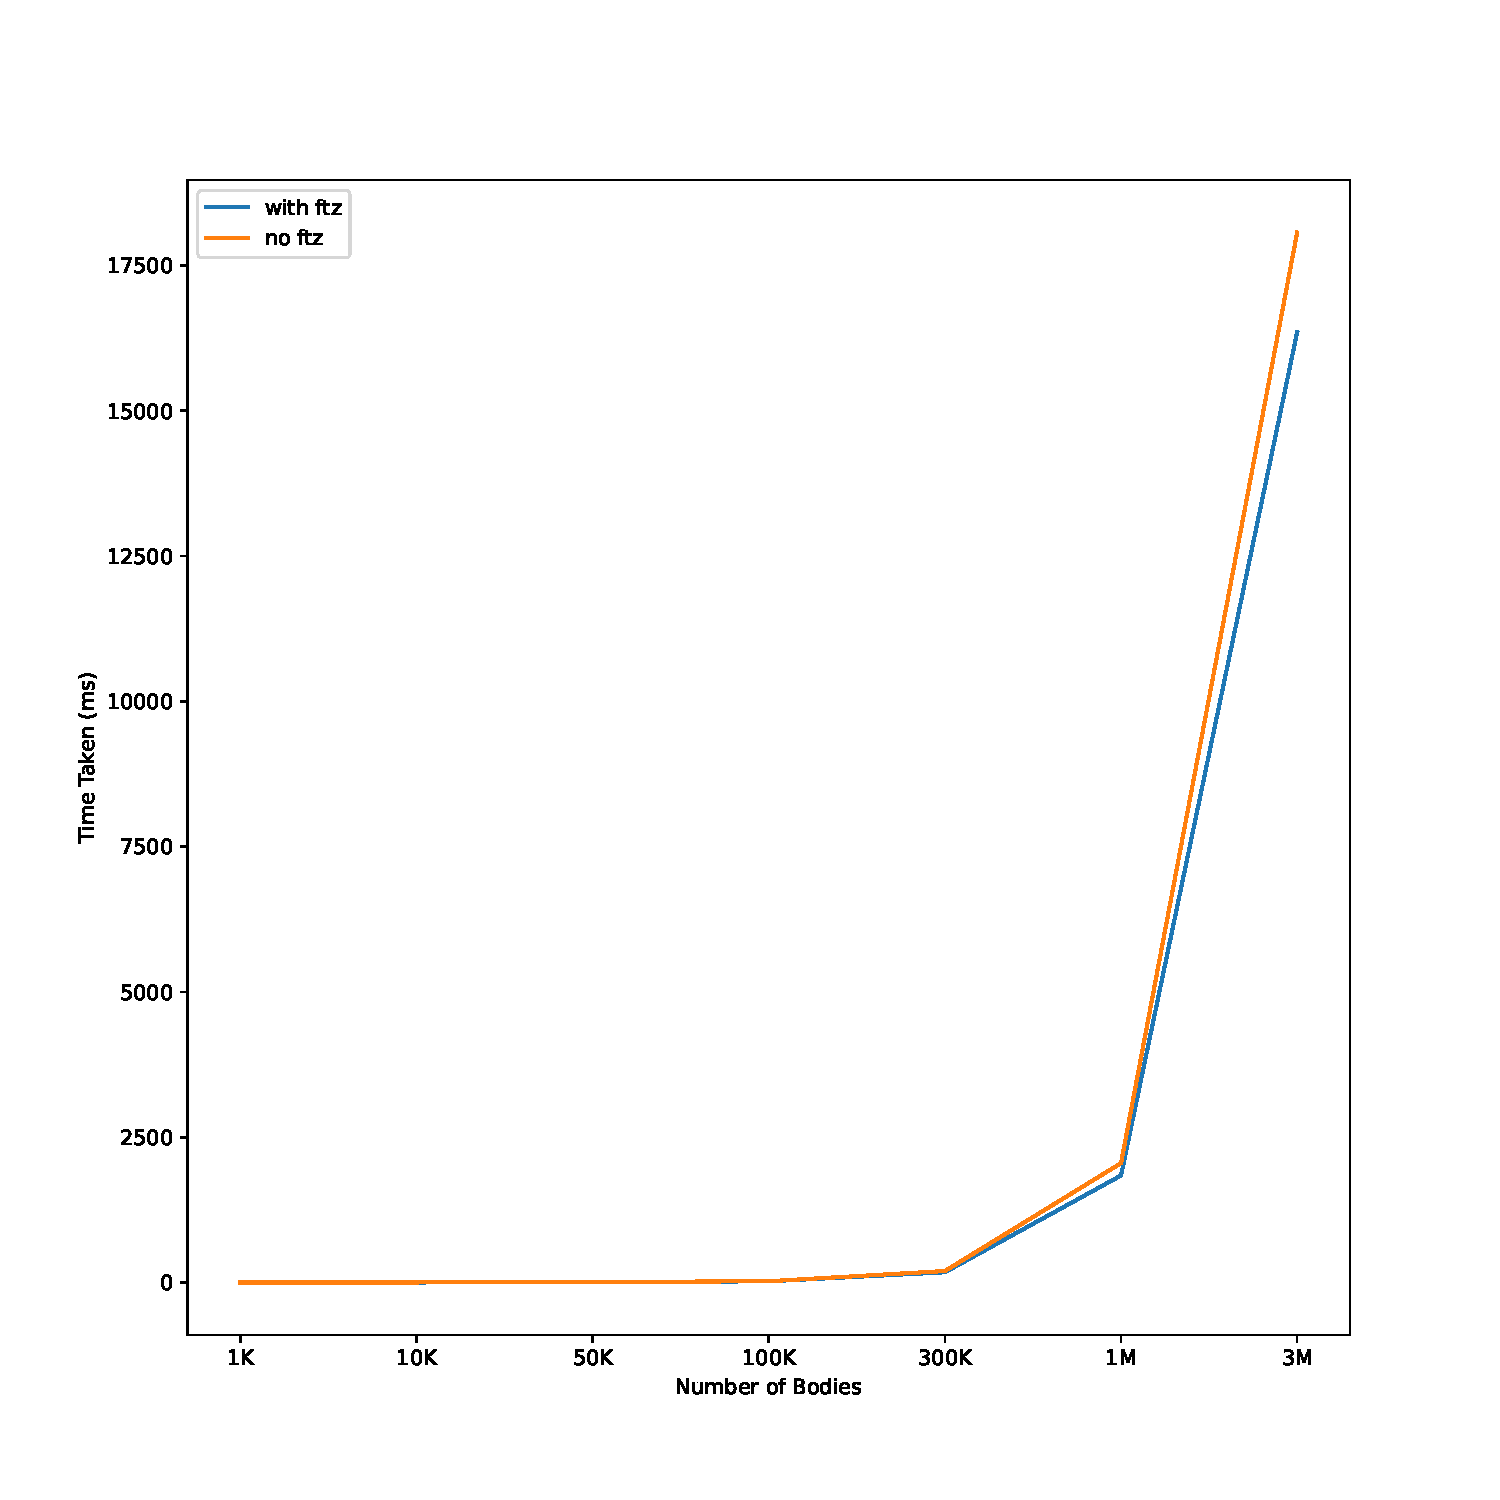
\includegraphics[width=0.7\textwidth]{Figures/graphs/ftz_cmp.pdf}}%
    \caption{Time Difference when using -ftz=true}
    \label{fig:swappinggggggg}
    
\end{figure}

\section{Discussion}
what was cool about this brah?
what could i do different or add to this and stuff yeah
any limits bro?

\section{Conclusion}
gpu rules parallelism is great yeah i be balling uh-huh yeah
